\chapter{Interoperability}
Merkle proofs from \ref{merkle:inclusion} are used to prove to a light client that a transaction has happened. \\
\textbf{Now this can be used to prove to blockchain B that a transaction like a token transfer has taken place in a blockchain A.}

In this chapter let's see how interoperability between blockchains can be achieved using merkle proofs. 

\section{Interoperability with merkle proofs}

\section{Examples}
So, now that we understand the merkle proofs, \textbf{how are they used in current interoperability solutions?}
\\We present a rapid overview of some interesting solutions, the goal here is to understand where the merkle proofs step in and how they help achieving interoperability in these protocols, leaving many details uncovered to keep it simple.
\subsection{LayerZero}
\begin{figure}[H]
    \centering
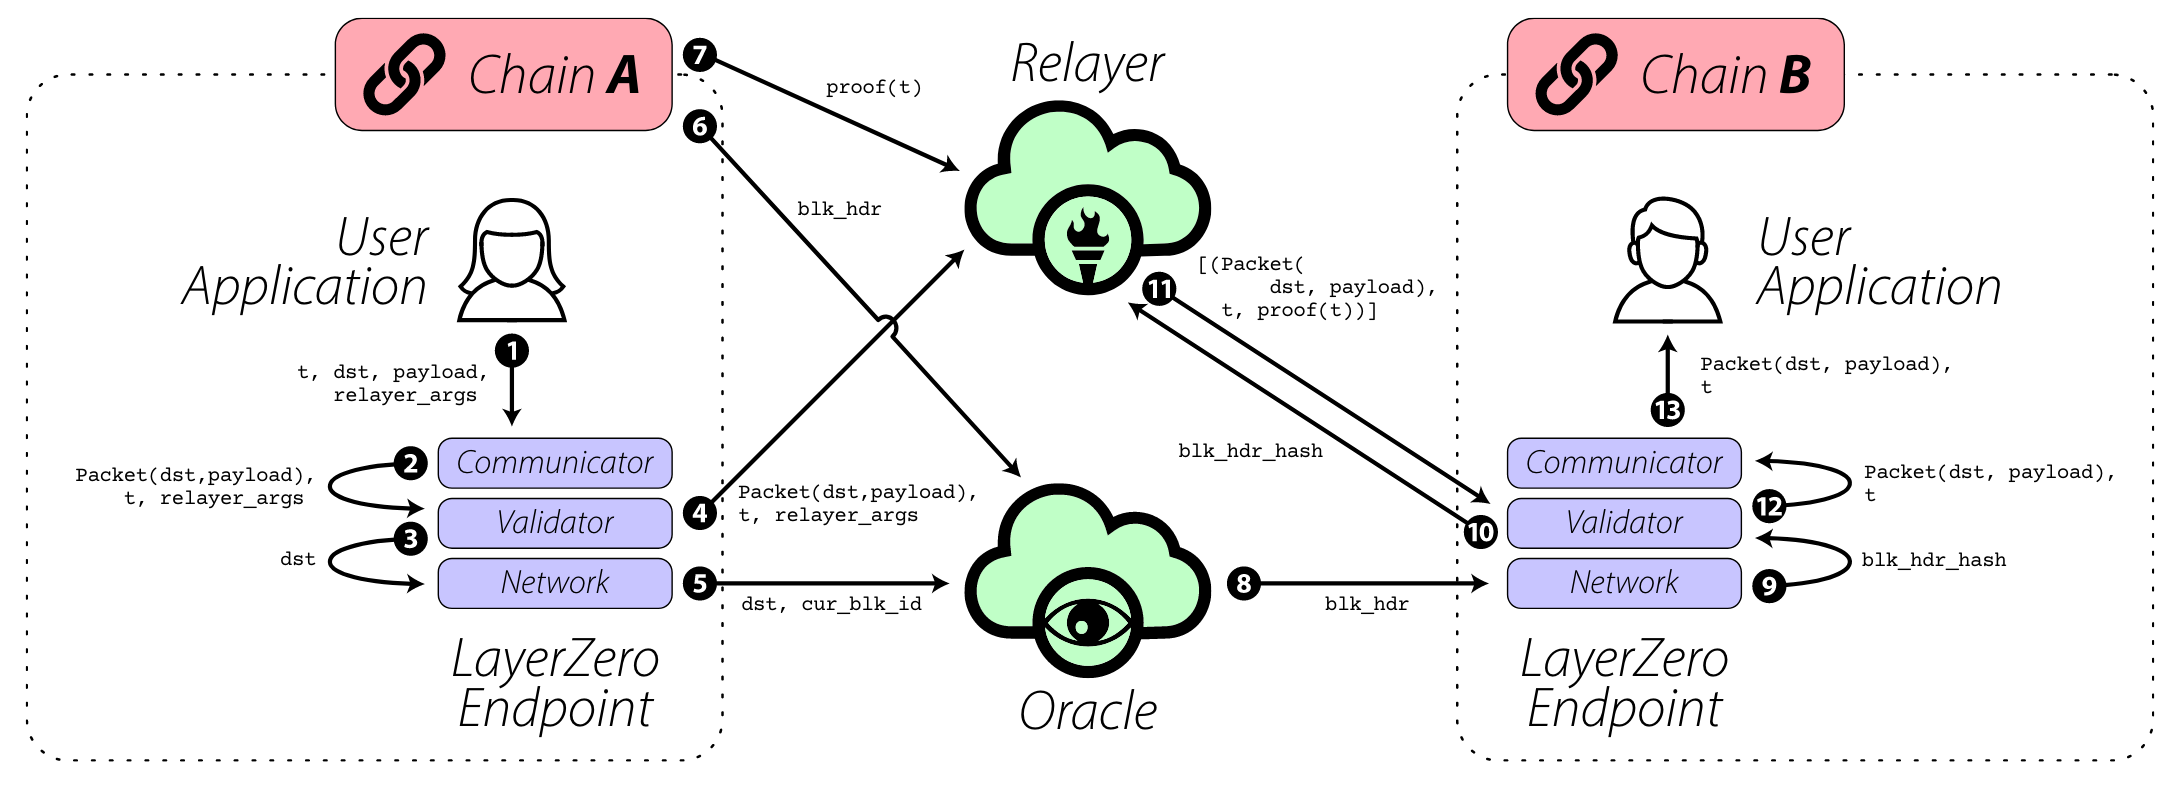
\includegraphics[width=1.\linewidth]{interoperability/layerZero.png}
    \caption{LayerZero}
    \label{fig:layer_zero}
\end{figure}

For each supported chain, LayerZero deploys an endpoint, consisting in 4 smart contracts. This endpoint includes a library handling the verification of the transaction proof.

So, from \ref{merkle:inclusion},  to verify that a transaction has taken place we need the merkle root, included in the block header and the the merkle proof. 
\\
LayerZero offers interoperability by transporting these two necessary pieces of data.
\begin{itemize}
    \item The block header containing the merkle root is carried by the oracle from blockchain A to blockchain B. 
    \item The merkle proof of blockchain A is carried by a relayer from blockchain A to blockchain B.
\end{itemize}

The oracle is a Chainlink oracle monitoring the source blockchain and the relayer can be handled by LayerZero or anyone interested into this. 
\\
Chain B can then attest that the transaction has happened by verifying the proof against the block header sent by the oracle.

\textbf{The security of LayerZero relies on the independence of the relayer and the oracle.}

If the oracle and the relayer collude, they can give a fake block header, and a proof working with that fake block. 


\subsection{ZKBridge}
\begin{figure}[H]
    \centering
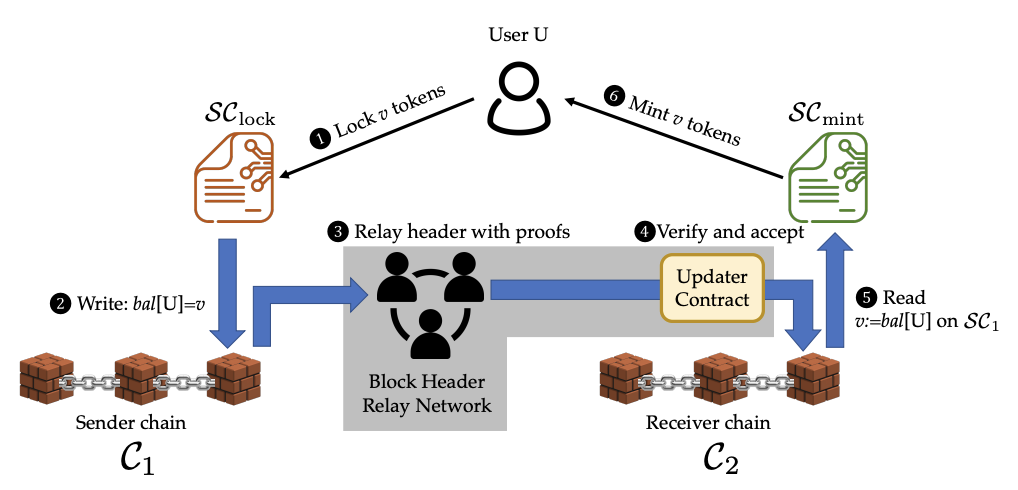
\includegraphics[width=0.8\linewidth]{interoperability/zkbridge.png}
    \caption{ZKbridge}
    \label{fig:zkbridge}
\end{figure}

So here, the gray part is ZKbridge.
\\The most important part is done here by the relayers. 
\begin{enumerate}
    \item The relayers contact the full nodes of blockchain C1 to get the last block header% $blkH_r$ following the $blkH_{r-1}$
    \item the relayers generate a zero knowledge proof that a light client of the sender chain C1 accepted that block header
    \item This proof is then sent to the ZKBridge updater contract of the receiving chain C2
    \item this updater contract verifies the ZK proof and adds it to its list of block headers if successfully verified.
    \item The application contract, anyone on C2 can call the public function GetHeader from the updater contract to get the header. 
\end{enumerate}

\textbf{The security of the ZKbridge relies notably on the security of the light client of C1.} It's because the zero knowledge proof consists in proving that this light client accepts the block.
\subsection{Telepathy}

\begin{figure}[H]
    \centering
    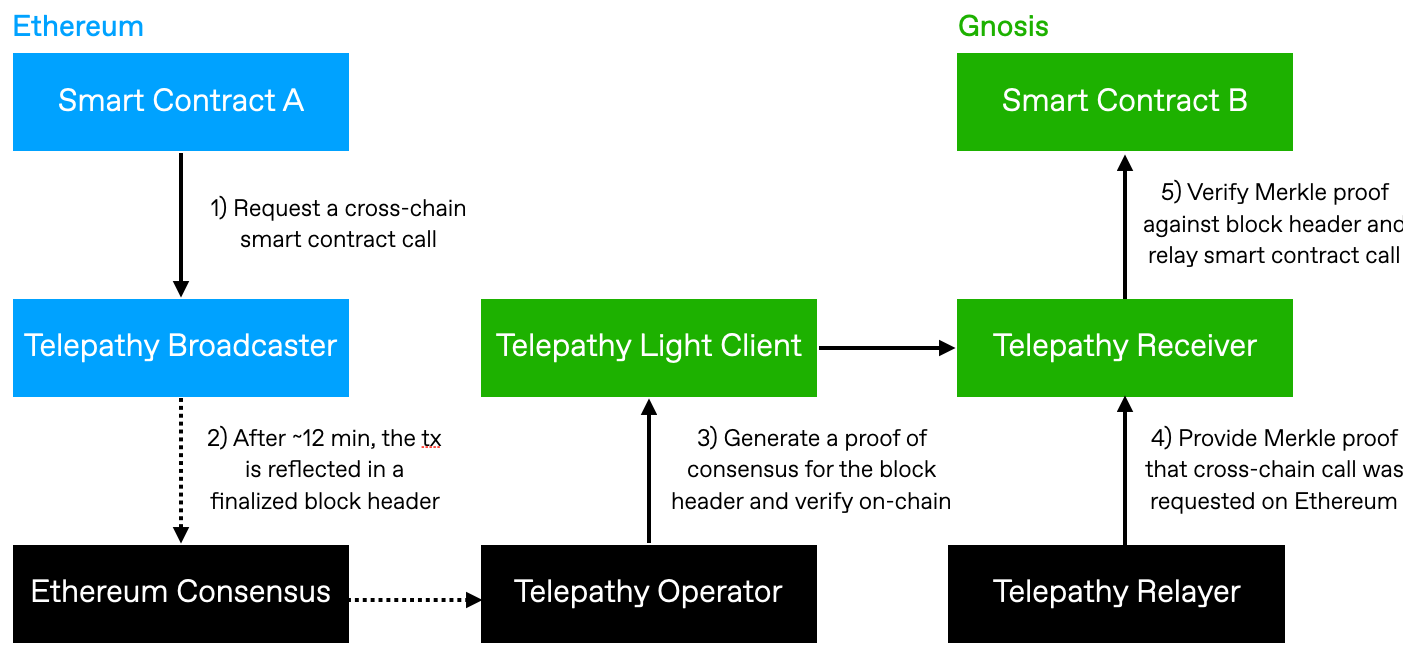
\includegraphics[width=0.8\linewidth]{interoperability/telepathy.png}
    \caption{Telepathy}
    \label{fig:telepathy}
\end{figure}

Telepathy is based on proof of consensus. It means that to prove that a block header from blockchain A is valid, it will basically check that a large majority of the validators signed the block header. But verifying all these signatures one by one is computationally expensive. Instead the proof used in Telepathy is a zero knowledge proof attesting that the block header has been signed by a sufficient percentage of validators. 

\textbf{The security of the Telepathy relies on the security of the underlying chain.}
\subsection{Axelar}

\subsection{Cosmos}